\documentclass{article}
\usepackage[T1]{fontenc}
\usepackage[polish]{babel}
\usepackage[utf8]{inputenc}
\usepackage{hyperref}
\usepackage{geometry}
 \geometry{
 a4paper,
 total={170mm,257mm},
 left=20mm,
 top=20mm,
 }
\usepackage{alltt}
\usepackage{listings} 
\lstset{language=Python, 
        basicstyle=\ttfamily\small, 
        keywordstyle=\color{keywords},
        commentstyle=\color{comments},
        stringstyle=\color{red},
        showstringspaces=false,
        identifierstyle=\color{green},
        keywords=[2]{pow},
        frame = single,
        keywordstyle=[2]{\color{orange}},
} 
\lstnewenvironment{code}{%
  \lstset{backgroundcolor=\color{verbgray},
  frame=single,
  framerule=0pt,
  basicstyle=\ttfamily,
  columns=fullflexible}}{}
\usepackage{pdfpages}
\usepackage{xcolor}
\usepackage{graphicx}
\usepackage{fancyvrb}
\usepackage{amsfonts}
\usepackage{stmaryrd}
\usepackage{amsmath}
\usepackage{psfrag}
\usepackage{wrapfig}
\usepackage{framed, color}
\definecolor{shadecolor}{rgb}{1., 0.8, 0.3}
\newcommand{\hlc}[2][shadecolor]{ 	{\sethlcolor{#1} \hl{#2}} }
\usepackage{fancyvrb}
\graphicspath{ {./images/} }
\definecolor{keywords}{RGB}{255,0,90}
\definecolor{comments}{RGB}{0,0,113}
\definecolor{red}{RGB}{160,0,0}
\definecolor{green}{RGB}{0,150,0} 
\usepackage{enumitem}
\usepackage{fancyhdr}
\cfoot{Programowanie aplikacji sieciowych, część 1 | Katarzyna Mazur}
\renewcommand{\footrulewidth}{0.4pt}
\fancyfoot[LE,RO]{\thepage}
\pagestyle{fancy}
\setcounter{tocdepth}{4}
\setcounter{secnumdepth}{4}
\usepackage{color,soul}
\definecolor{verbgray}{gray}{0.9}

\title{Programowanie aplikacji sieciowych \\ \small Zbiór zadań, część pierwsza}
\date{}
\author{Katarzyna Mazur}

\begin{document}

\maketitle
\newpage

\tableofcontents

\newpage

\section*{Gniazda w języku Python - moduł socket} \mbox{}\\

\noindent \textbf{Tworzenie gniazd klienckich/serwerowych TCP, IPv4}

\begin{code}
#!/usr/bin/env python3
import socket

if __name__ == '__main__':

	sockIPv4 = socket.socket(socket.AF_INET, socket.SOCK_STREAM)
	sockIPv4.close()
\end{code} \mbox{}\\

\noindent \textbf{Tworzenie gniazd klienckich/serwerowych TCP, IPv6}

\begin{code}
#!/usr/bin/env python3
import socket

if __name__ == '__main__':

	sockIPv6 = socket.socket(socket.AF_INET6, socket.SOCK_STREAM)
	sockIPv6.close()
\end{code} \mbox{}\\

\noindent \textbf{Tworzenie gniazd klienckich/serwerowych UDP, IPv4}

\begin{code}
#!/usr/bin/env python3
import socket 

if __name__ == '__main__':

	sockIPv4 = socket.socket(socket.AF_INET,  socket.SOCK_DGRAM)
	sockIPv4.close()
\end{code}\mbox{}\\

\noindent \textbf{Tworzenie gniazd klienckich/serwerowych UDP, IPv6}

\begin{code}
#!/usr/bin/env python3
import socket 

if __name__ == '__main__':

	sockIPv6 = socket.socket(socket.AF_INET6,  socket.SOCK_DGRAM)
	sockIPv6.close()
\end{code}\mbox{}\\

\newpage
\noindent \textbf{Gniazdo klienckie TCP, IPv4: nawiązanie połączenia z serwerem}

\begin{code}
#!/usr/bin/env python3
import socket

if __name__ == "__main__":

    sockIPv4 = socket.socket(socket.AF_INET, socket.SOCK_STREAM)
    sockIPv4.settimeout(5)

    try:
        sockIPv4.connect(("127.0.0.1", 80))
    except socket.error as exc:
        print(f"Wyjatek socket.error: {exc}")

    sockIPv4.close()
\end{code}\mbox{}\\


\noindent \textbf{Gniazdo klienckie TCP, IPv6: nawiązanie połączenia z serwerem}

\begin{code}
#!/usr/bin/env python3
import socket

if __name__ == "__main__":

    address = socket.getaddrinfo("::1", 80, socket.AF_INET6)
    sockIPv6 = socket.socket(socket.AF_INET6, socket.SOCK_STREAM)
    sockIPv6.settimeout(5)

    try:
        sockIPv6.connect(address[0][4])
    except socket.error as exc:
        print(f"Wyjatek socket.error: {exc}")

    sockIPv6.close()
\end{code}\mbox{}\\

\noindent \textbf{Gniazdo klienckie TCP, IPv4: komunikacja z serwerem (wysyłanie i odbieranie danych)}

\begin{code}
#!/usr/bin/env python3
import socket

if __name__ == "__main__":

    sockIPv4 = socket.socket(socket.AF_INET, socket.SOCK_STREAM)
    sockIPv4.settimeout(5)

    try:
        sockIPv4.connect(("127.0.0.1", 80))
        sockIPv4.sendall("Hello Server!".encode())	# wysylanie
        print(sockIPv4.recv(1024).decode())								# odbieranie
    except socket.error as exc:
        print(f"Wyjatek socket.error: {exc}")

    sockIPv4.close()
\end{code}\mbox{}\\

\newpage
\noindent \textbf{Gniazdo klienckie TCP, IPv6: komunikacja z serwerem (wysyłanie i odbieranie danych)}

\begin{code}
#!/usr/bin/env python3
import socket

if __name__ == "__main__":

    address = socket.getaddrinfo("::1", 80, socket.AF_INET6)
    sockIPv6 = socket.socket(socket.AF_INET6, socket.SOCK_STREAM)
    sockIPv6.settimeout(5)

    try:
        sockIPv6.connect(address[0][4])
        sockIPv6.sendall("Hello Server!".encode())	# wysylanie
        print(sockIPv6.recv(1024).decode())								# odbieranie
    except socket.error as exc:
        print(f"Wyjatek socket.error: {exc}")

    sockIPv6.close()
\end{code}\mbox{}\\

\noindent \textbf{Gniazdo klienckie UDP, IPv4: komunikacja z serwerem (wysyłanie i odbieranie danych)}

\begin{code}
#!/usr/bin/env python3

import socket

HOST = '127.0.0.1'
PORT = 80

sockIPv4 = socket.socket(socket.AF_INET, socket.SOCK_DGRAM)
server_address = (HOST, PORT)

try:
    message = "Hello Server!"
    sent = sockIPv4.sendto(message.encode(), server_address)		# wysylanie
    data, server = sockIPv4.recvfrom(4096)																				# odbieranie
    print(f"Received: {data.decode()}")

finally:
    sockIPv4.close()
\end{code}\mbox{}\\

\noindent \textbf{Gniazdo klienckie UDP, IPv6: komunikacja z serwerem (wysyłanie i odbieranie danych)}

\begin{code}
#!/usr/bin/env python3

import socket

HOST = "::1"
PORT = 80

sockIPv6 = socket.socket(socket.AF_INET6, socket.SOCK_DGRAM)

try:
    sockIPv6.sendto("Hello Server!".encode(), (HOST, PORT))			# wysylanie
    data, server = sockIPv6.recvfrom(4096)																				# odbieranie
    print(f"Received: {data.decode()}")

finally:
    sockIPv6.close()
\end{code}



\newpage 
\section{Zadania wprowadzające}

\begin{enumerate}[label=\textbf{1.\arabic*}]\setlength{\itemsep}{1em}
    \item  Napisz program, w którym pobierzesz od użytkownika nazwę pliku tekstowego w formacie \texttt{*.txt}, a następnie skopiujesz go do pliku pod nazwą \texttt{lab1zad1.txt}. Zadbaj o prawidłową obsługę błędów.
    \item Napisz program, w którym pobierzesz od użytkownika nazwę pliku graficznego w formacie \texttt{*.png}, a następnie skopiujesz go do pliku pod nazwą \texttt{lab1zad2.png}. Zadbaj o prawidłową obsługę błędów.
    \item Napisz program, w którym pobierzesz od użytkownika adres \texttt{IPv4}, a następnie sprawdzisz, czy jest on prawidłowym adresem. Zadbaj o prawidłową obsługę błędów. \textit{Podpowiedź: zadanie możesz rozwiązać przy pomocy wyrażeń regularnych}
    \item Napisz program, w którym pobierzesz od użytkownika adres \texttt{IPv6}, a następnie sprawdzisz, czy jest on prawidłowym adresem.  Zadbaj o prawidłową obsługę błędów. \textit{Podpowiedź: zadanie możesz rozwiązać przy pomocy wyrażeń regularnych}
    \item Napisz program, który jako argument linii poleceń pobierze od użytkownika adres \texttt{IPv4}, a następnie wyświetli odpowiadającą mu nazwę \texttt{hostname} (nazwę domenową). Zadanie rozwiąż bez użycia dodatkowych bibliotek. Zadbaj o prawidłową obsługę błędów.
\end{enumerate}

\newpage 
\section{Analiza pakietów sieciowych}

\begin{enumerate}[label=\textbf{2.\arabic*}]\setlength{\itemsep}{1em}
    \item \label{ex21} Poniżej znajduje się pełny zapis datagramu UDP w postaci szesnastkowej. \\

\begin{figure}[h!t!p!]
\centering
\begin{BVerbatim}
ed 74 0b 55 00 24 ef fd 70 72 6f 67 72 61
6d 6d 69 6e 67 20 69 6e 20 70 79 74 68 6f 
6e 20 69 73 20 66 75 6e
\end{BVerbatim}
\end{figure}

\noindent  Wiedząc, że w zapisie szesnastkowym jedna cyfra reprezentuje $4$ bity, oraz znając strukturę datagramu UDP: 

\begin{figure}[ht!]
\centering
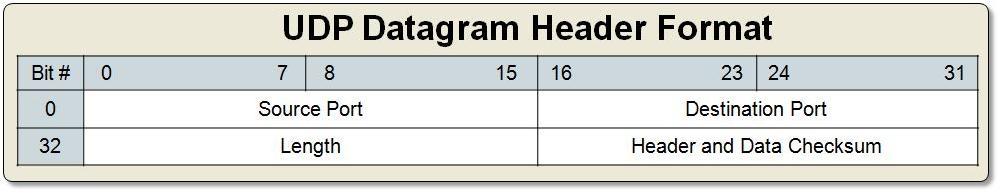
\includegraphics[scale=0.5]{/ch2/udp.jpg}
\end{figure}

\noindent Napisz program, który z powyższego datagramu UDP wydobędzie: 

\begin{itemize}
\item numer źródłowego portu
\item numer docelowego portu
\item dane (ile bajtów w tym pakiecie zajmują dane?)
\end{itemize}

\noindent A następnie uzyskany wynik w postaci: \hlc[shadecolor]{ zad2.1odp;src;X;dst;Y;data;Z } gdzie:

\begin{itemize}
\item X to wydobyty z pakietu numer portu źródłowego
\item Y to wydobyty z pakietu numer portu docelowego
\item Z to wydobyte z pakietu dane 
\end{itemize}

 prześle do serwera UDP działającego na wskazanym porcie pod podanym adresem IPv4, w celu sprawdzenia, czy udało się prawidłowo odczytać wymagane pola. Serwer zwróci odpowiedź \texttt{TAK} lub \texttt{NIE}, a w przypadku błędnego sformatowania wiadomości, odeśle odpowiedź \texttt{BAD\_SYNTAX}.  Podczas pisania kodu związanego z operacjami sieciowymi, nie korzystaj z dodatkowych bibliotek, wykorzystaj jedynie gniazda. Zadbaj o prawidłową obsługę błędów. 

 % ####################################################################################################################  
  \item Zmodyfikuj program z zadania \ref{ex21} w taki sposób,  aby łączył się z serwerem posiadającym adres IPv6.  Adres IPv6 serwera i numer portu pobierz jako argumenty linii poleceń. Podczas pisania kodu związanego z operacjami sieciowymi, nie korzystaj z dodatkowych bibliotek, wykorzystaj jedynie gniazda. Zadbaj o prawidłową obsługę błędów. 
 

% ####################################################################################################################  
 \item \label{ex22} Poniżej znajduje się pełny zapis segmentu TCP w postaci szesnastkowej (pole opcji ma 12 bajtów). \\ 

\begin{figure}[h!t!p!]
\centering
\begin{BVerbatim}
0b 54 89 8b 1f 9a 18 ec bb b1 64 f2 80 18
00 e3 67 71 00 00 01 01 08 0a 02 c1 a4 ee 
00 1a 4c ee 68 65 6c 6c 6f 20 3a 29
\end{BVerbatim}
\end{figure}\mbox{}

\noindent  Wiedząc, że w zapisie szesnastkowym jedna cyfra reprezentuje $4$ bity, oraz znając strukturę segmentu TCP:\\

\begin{figure}[ht!]
\centering
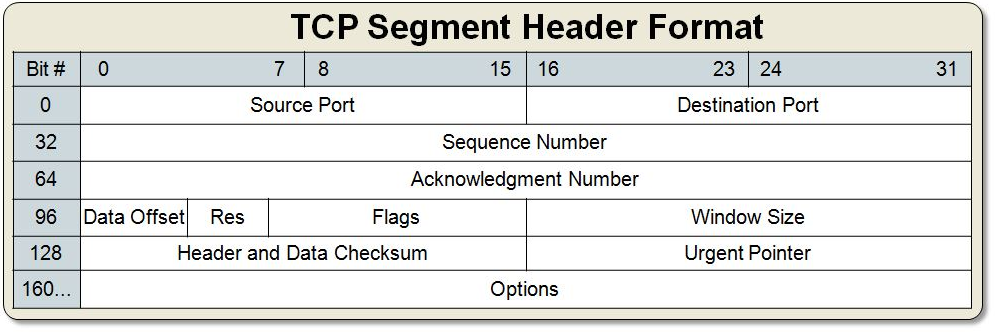
\includegraphics[scale=0.45]{./ch2/tcp.png}
\end{figure}
\newpage 
\noindent Napisz program, który z powyższego segmentu TCP wydobędzie: 

\begin{itemize}
\item numer źródłowego portu
\item numer docelowego portu
\item dane (ile bajtów w tym pakiecie zajmują dane?)
\end{itemize}

\noindent A następnie uzyskany wynik w postaci: \hlc[shadecolor]{ zad2.3odp;src;X;dst;Y;data;Z } gdzie:

\begin{itemize}
\item X to wydobyty z pakietu numer portu źródłowego
\item Y to wydobyty z pakietu numer portu docelowego
\item Z to wydobyte z pakietu dane 
\end{itemize}

 prześle do serwera TCP działającego na wskazanym porcie pod podanym adresem IPv4, w celu sprawdzenia, czy udało się prawidłowo odczytać wymagane pola. Serwer zwróci odpowiedź \texttt{TAK} lub \texttt{NIE}, a w przypadku błędnego sformatowania wiadomości, odeśle odpowiedź \texttt{BAD\_SYNTAX}.  Podczas pisania kodu związanego z operacjami sieciowymi, nie korzystaj z dodatkowych bibliotek, wykorzystaj jedynie gniazda. Zadbaj o prawidłową obsługę błędów. 
% ####################################################################################################################  
 

  \item Zmodyfikuj program z zadania \ref{ex22} w taki sposób,  aby łączył się z serwerem posiadającym adres IPv6.  Adres IPv6 serwera i numer portu pobierz jako argumenty linii poleceń. Podczas pisania kodu związanego z operacjami sieciowymi, nie korzystaj z dodatkowych bibliotek, wykorzystaj jedynie gniazda. Zadbaj o prawidłową obsługę błędów. 

\end{enumerate}

\newpage
\section{Gniazda klienckie}

\subsection*{Gniazda TCP}

\begin{enumerate}[label=\textbf{3.\arabic*}]\setlength{\itemsep}{1em}
    \item \label{ex31} Napisz program klienta, w którym połączysz się z serwerem na danym porcie przy użyciu protokołu TCP. Adres IPv4 serwera i numer portu pobierz jako argumenty linii poleceń. Wyświetl informację, czy udało się nawiązać połączenie. Program powinien akceptować adres w postaci adresu IPv4 jak i hostname. Podczas pisania kodu związanego z operacjami sieciowymi, nie korzystaj z dodatkowych bibliotek, wykorzystaj jedynie gniazda. Zadbaj o prawidłową obsługę błędów. 
    
    \item Zmodyfikuj program z zadania \ref{ex31} w taki sposób, aby łączył się z serwerem posiadającym adres IPv6.  Adres IPv6 serwera i numer portu pobierz jako argumenty linii poleceń. Podczas pisania kodu związanego z operacjami sieciowymi, nie korzystaj z dodatkowych bibliotek, wykorzystaj jedynie gniazda. Zadbaj o prawidłową obsługę błędów. 
    
    \item \label{ex33} Napisz program klienta (prosty skaner portów sieciowych), który dla danego serwera przy użyciu protokołu TCP będzie sprawdzał, jakie porty są otwarte, a jakie zamknięte. Adres IPv4 serwera pobierz jako argument linii poleceń. Program powinien akceptować adres w postaci adresu IPv4 jak i hostname.  Podczas pisania kodu związanego z operacjami sieciowymi, nie korzystaj z dodatkowych bibliotek, wykorzystaj jedynie gniazda. Zadbaj o prawidłową obsługę błędów. 
    
    \item  Zmodyfikuj program z zadania \ref{ex33} w taki sposób,  aby łączył się z serwerem posiadającym adres IPv6.  Adres IPv6 serwera i numer portu pobierz jako argumenty linii poleceń. Podczas pisania kodu związanego z operacjami sieciowymi, nie korzystaj z dodatkowych bibliotek, wykorzystaj jedynie gniazda. Zadbaj o prawidłową obsługę błędów. 
    
    \item \label{ex35} Napisz program klienta, który z serwera o podanym adresie IPv4 i porcie pobierze aktualną datę i czas, a następnie wyświetli je na konsoli.  Adres IPv4 serwera i numer portu pobierz jako argumenty linii poleceń. Podczas pisania kodu związanego z operacjami sieciowymi, nie korzystaj z dodatkowych bibliotek, wykorzystaj jedynie gniazda. Zadbaj o prawidłową obsługę błędów. 
    
     \item Zmodyfikuj program z zadania \ref{ex35} w taki sposób,  aby łączył się z serwerem posiadającym adres IPv6.  Adres IPv6 serwera i numer portu pobierz jako argumenty linii poleceń. Podczas pisania kodu związanego z operacjami sieciowymi, nie korzystaj z dodatkowych bibliotek, wykorzystaj jedynie gniazda. Zadbaj o prawidłową obsługę błędów. 
     
     \item \label{ex37} Napisz program klienta, który połączy się z serwerem TCP działającym pod podanym adresem IPv4 na podanym porcie, a następnie wyśle do niego wiadomość i odbierze odpowiedź.  Adres IPv4 serwera i numer portu pobierz jako argumenty linii poleceń. Podczas pisania kodu związanego z operacjami sieciowymi, nie korzystaj z dodatkowych bibliotek, wykorzystaj jedynie gniazda. Zadbaj o prawidłową obsługę błędów. 
     
     \item Zmodyfikuj program z zadania \ref{ex37} w taki sposób,  aby łączył się z serwerem posiadającym adres IPv6.  Adres IPv6 serwera i numer portu pobierz jako argumenty linii poleceń. Podczas pisania kodu związanego z operacjami sieciowymi, nie korzystaj z dodatkowych bibliotek, wykorzystaj jedynie gniazda. Zadbaj o prawidłową obsługę błędów. 
     
     \item \label{ex39} Napisz program klienta, który połączy się z serwerem TCP działającym pod podanym adresem IPv4 na podanym porcie,  a następnie będzie w pętli wysyłał do niego tekst wczytany od użytkownika (jako argument wywołania programu bądź jako dane podawane na konsoli), i odbierał odpowiedzi.  Adres IPv4 serwera i numer portu pobierz jako argumenty linii poleceń. Podczas pisania kodu związanego z operacjami sieciowymi, nie korzystaj z dodatkowych bibliotek, wykorzystaj jedynie gniazda. Zadbaj o prawidłową obsługę błędów. 
     
     \item Zmodyfikuj program z zadania \ref{ex39} w taki sposób,  aby łączył się z serwerem posiadającym adres IPv6.  Adres IPv6 serwera i numer portu pobierz jako argumenty linii poleceń. Podczas pisania kodu związanego z operacjami sieciowymi, nie korzystaj z dodatkowych bibliotek, wykorzystaj jedynie gniazda. Zadbaj o prawidłową obsługę błędów. 

    \item  \label{ex311} Napisz program klienta (prosty skaner portów sieciowych), który dla danego serwera przy użyciu protokołu TCP będzie sprawdzał, jakie porty są otwarte, a jakie zamknięte. Oprócz informacji o otwartych / zamkniętych portach, program powinien również wyświetlać informację o tym, jaka usługa jest uruchomiona na danym porcie (baner usługi).  Adres IPv4 serwera pobierz jako argument linii poleceń. Program powinien akceptować adres w postaci adresu IPv4 jak i hostname.  Podczas pisania kodu związanego z operacjami sieciowymi, nie korzystaj z dodatkowych bibliotek, wykorzystaj jedynie gniazda. Zadbaj o prawidłową obsługę błędów.  
    
    \item Zmodyfikuj program z zadania \ref{ex311} w taki sposób,  aby łączył się z serwerem posiadającym adres IPv6. Podczas pisania kodu związanego z operacjami sieciowymi, nie korzystaj z dodatkowych bibliotek, wykorzystaj jedynie gniazda. Zadbaj o prawidłową obsługę błędów. 
    
    \item \label{ex313} Napisz program klienta, który połączy się z serwerem TCP działającym pod podanym adresem IPv4 na podanym porcie, a następnie wyśle do niego wiadomość i odbierze odpowiedź. Warunkiem zadania jest, aby klient wysłał i odebrał od serwera wiadomość o maksymalnej długości 20 znaków. Podczas pisania kodu związanego z operacjami sieciowymi, nie korzystaj z dodatkowych bibliotek, wykorzystaj jedynie gniazda. Zadbaj o prawidłową obsługę błędów.  Uwzględnij sytuacje, gdy:
    \begin{itemize}
    \item wiadomość do wysłania jest za krótka - ma być wówczas uzupełniania do 20 znaków znakami spacji
    \item wiadomość do wysłania jest za długa - ma być przycięta do 20 znaków (lub wysłana w całości - sprawdź, co się wówczas stanie)
    \end{itemize}
    
    \item Zmodyfikuj program z zadania \ref{ex313} w taki sposób,  aby łączył się z serwerem posiadającym adres IPv6. Podczas pisania kodu związanego z operacjami sieciowymi, nie korzystaj z dodatkowych bibliotek, wykorzystaj jedynie gniazda. Zadbaj o prawidłową obsługę błędów. 
    
    \item \label{ex315} Dostępne dla gniazd funkcje \texttt{recv} i \texttt{send} nie gwarantują wysłania / odbioru wszystkich danych. Rozważmy funkcję \texttt{recv}. Przykładowo, $100$ bajtów może zostać wysłane jako grupa po $10$ bajtów, albo od razu w całości. Oznacza to, iż jeśli używamy gniazd TCP, musimy odbierać dane, dopóki nie mamy pewności, że odebraliśmy odpowiednią ich ilość. Napisz program klienta, który połączy się z serwerem TCP działającym pod podanym adresem IPv4 na podanym porcie, a następnie wyśle do niego wiadomość i odbierze odpowiedź. Dane odbieraj / wysyłaj w ten sposób, aby mieć pewność, że klient w rzeczywistości odebrał / wysłał wiadomość o wymaganej długości. Podczas pisania kodu związanego z operacjami sieciowymi, nie korzystaj z dodatkowych bibliotek, wykorzystaj jedynie gniazda. Zadbaj o prawidłową obsługę błędów. 
    
    \item Zmodyfikuj program z zadania \ref{ex315} w taki sposób,  aby łączył się z serwerem posiadającym adres IPv6. Podczas pisania kodu związanego z operacjami sieciowymi, nie korzystaj z dodatkowych bibliotek, wykorzystaj jedynie gniazda. Zadbaj o prawidłową obsługę błędów. 
   
\end{enumerate}

\subsection*{Gniazda UDP}

\begin{enumerate}[label=\textbf{3.\arabic*}, resume]\setlength{\itemsep}{1em}

\item \label{ex317}  Napisz program klienta, który połączy się z serwerem UDP działającym pod podanym adresem IPv4 na podanym porcie, a następnie wyśle do niego wiadomość i odbierze odpowiedź. Adres IPv4 serwera oraz numer portu pobierz jako argumenty linii poleceń. Program powinien akceptować adres w postaci adresu IPv4 jak i hostname.  Podczas pisania kodu związanego z operacjami sieciowymi, nie korzystaj z dodatkowych bibliotek, wykorzystaj jedynie gniazda. Zadbaj o prawidłową obsługę błędów.  

\item  Zmodyfikuj program z zadania \ref{ex317} w taki sposób,  aby łączył się z serwerem posiadającym adres IPv6.  Adres IPv6 serwera i numer portu pobierz jako argumenty linii poleceń. Podczas pisania kodu związanego z operacjami sieciowymi, nie korzystaj z dodatkowych bibliotek, wykorzystaj jedynie gniazda. Zadbaj o prawidłową obsługę błędów. 

\item \label{ex319} Napisz program klienta, który połączy się z serwerem UDP działającym pod podanym adresem IPv4 na podanym porcie,  a następnie będzie w pętli wysyłał do niego tekst wczytany od użytkownika, i odbierał odpowiedzi.    Adres IPv4 serwera i numer portu pobierz jako argumenty linii poleceń. Podczas pisania kodu związanego z operacjami sieciowymi, nie korzystaj z dodatkowych bibliotek, wykorzystaj jedynie gniazda. Zadbaj o prawidłową obsługę błędów. 

\item  Zmodyfikuj program z zadania \ref{ex319} w taki sposób,  aby łączył się z serwerem posiadającym adres IPv6. Adres IPv6 serwera i numer portu pobierz jako argumenty linii poleceń. Podczas pisania kodu związanego z operacjami sieciowymi, nie korzystaj z dodatkowych bibliotek, wykorzystaj jedynie gniazda. Zadbaj o prawidłową obsługę błędów. 

\item \label{ex321} Napisz program klienta, który połączy się z serwerem UDP działającym pod podanym adresem IPv4 na podanym porcie, a następnie prześle do serwera liczbę, operator, liczbę (pobrane od użytkownika) i odbierze odpowiedź. Adres IPv4 serwera i numer portu pobierz jako argumenty linii poleceń.  Podczas pisania kodu związanego z operacjami sieciowymi, nie korzystaj z dodatkowych bibliotek, wykorzystaj jedynie gniazda. Zadbaj o prawidłową obsługę błędów. 

\item  Zmodyfikuj program z zadania \ref{ex321} w taki sposób,  aby łączył się z serwerem posiadającym adres IPv6. Adres IPv6 serwera i numer portu pobierz jako argumenty linii poleceń. Podczas pisania kodu związanego z operacjami sieciowymi, nie korzystaj z dodatkowych bibliotek, wykorzystaj jedynie gniazda. Zadbaj o prawidłową obsługę błędów. 

\item \label{ex322} Napisz program klienta, który połączy się z serwerem UDP działającym pod podanym adresem IPv4 na podanym porcie, a następnie prześle do serwera pobrany z linii poleceń adres IP, i odbierze odpowiadającą mu nazwę hostname. Podczas pisania kodu związanego z operacjami sieciowymi, nie korzystaj z dodatkowych bibliotek, wykorzystaj jedynie gniazda. Zadbaj o prawidłową obsługę błędów. 

\item  Zmodyfikuj program z zadania \ref{ex322} w taki sposób,  aby łączył się z serwerem posiadającym adres IPv6. Adres IPv6 serwera i numer portu pobierz jako argumenty linii poleceń. Podczas pisania kodu związanego z operacjami sieciowymi, nie korzystaj z dodatkowych bibliotek, wykorzystaj jedynie gniazda. Zadbaj o prawidłową obsługę błędów. 

\item \label{ex323} Napisz program klienta, który połączy się z serwerem UDP działającym pod podanym adresem IPv4 na podanym porcie, a następnie prześle do serwera nazwę hostname pobraną z linii poleceń, i odbierze odpowiadający mu adres IP.  Podczas pisania kodu związanego z operacjami sieciowymi, nie korzystaj z dodatkowych bibliotek, wykorzystaj jedynie gniazda. Zadbaj o prawidłową obsługę błędów. 

\item Zmodyfikuj program z zadania \ref{ex323} w taki sposób,  aby łączył się z serwerem posiadającym adres IPv6. Adres IPv6 serwera i numer portu pobierz jako argumenty linii poleceń. Podczas pisania kodu związanego z operacjami sieciowymi, nie korzystaj z dodatkowych bibliotek, wykorzystaj jedynie gniazda. Zadbaj o prawidłową obsługę błędów. 
\end{enumerate}

\newpage
\section{Gniazda serwerowe}

\subsection*{Gniazda TCP}
\subsection*{Gniazda UDP}

\newpage
\section{Bezpiecznie gniazda}

\newpage
\section{Protokoły pocztowe}

\subsection*{Protokół SMTP}

\begin{enumerate}[label=\textbf{6.\arabic*}]\setlength{\itemsep}{1em}

\item Pod podanym adresem i numerem portu działa serwer obsługujący protokół ESMTP/SMTP. Wykorzystując gotowe oprogramowanie klienckie połącz się z serwerem działajacym pod podanym adresem i numerem portu, a następnie wyślij wiadomość e-mail korzytając z komend protokołu ESMTP.  (\textit{Zadanie nie jest zadaniem programistycznym, wymaga jedynie użycia gotowego klienta protokołu SMTP w celu zapoznania się z podstawowymi poleceniami protokołu.})

\item Pod podanym adresem i numerem portu działa serwer obsługujący protokół ESMTP/SMTP. Wykorzystując gotowe oprogramowanie klienckie połącz się z serwerem działajacym pod podanym adresem i numerem portu, a następnie wyślij kilka wiadomości e-mail do kilku odbiorców korzytając z komend protokołu ESMTP.  (\textit{Zadanie nie jest zadaniem programistycznym, wymaga jedynie użycia gotowego klienta protokołu SMTP w celu zapoznania się z podstawowymi poleceniami protokołu.})

\item Pod podanym adresem i numerem portu działa serwer obsługujący protokół ESMTP/SMTP. Wykorzystując gotowe oprogramowanie klienckie połącz się z serwerem działajacym pod podanym adresem i numerem portu, a następnie wyślij wiadomość spoofed e-mail (z podmienionym adresem nadawcy) korzytając z komend protokołu ESMTP.  (\textit{Zadanie nie jest zadaniem programistycznym, wymaga jedynie użycia gotowego klienta protokołu SMTP w celu zapoznania się z podstawowymi poleceniami protokołu.})

\item Pod podanym adresem i numerem portu działa serwer obsługujący protokół ESMTP/SMTP. Wykorzystując gotowe oprogramowanie klienckie połącz się z serwerem działajacym pod podanym adresem i numerem portu, a następnie wyślij wiadomość e-mail korzytając z komend protokołu ESMTP.  Do wiadomości dodaj załącznik - dowolny plik tekstowy (sprawdź format MIME: \href{https://www.w3.org/Protocols/rfc1341/7_2_Multipart.html}{Multipart} i \href{https://www.w3.org/Protocols/rfc1341/7_3_Message.html}{Content-Type}).  Możesz wykorzystać \texttt{openssl} do przekonwertowania pliku: \texttt{cat plik.txt \textbar  openssl base64}.  (\textit{Zadanie nie jest zadaniem programistycznym, wymaga jedynie użycia gotowego klienta protokołu SMTP w celu zapoznania się z podstawowymi poleceniami protokołu.})

\item Pod podanym adresem i numerem portu działa serwer obsługujący protokół ESMTP/SMTP. Wykorzystując gotowe oprogramowanie klienckie połącz się z serwerem działajacym pod podanym adresem i numerem portu, a następnie wyślij wiadomość e-mail korzytając z komend protokołu ESMTP. Do wiadomości dodaj załącznik - dowolny obrazek (sprawdź format MIME: \href{https://www.w3.org/Protocols/rfc1341/7_2_Multipart.html}{Multipart} i \href{https://www.w3.org/Protocols/rfc1341/7_3_Message.html}{Content-Type}). Możesz wykorzystać \texttt{openssl} do przekonwertowania obrazka: \texttt{cat obrazek \textbar  openssl base64}. (\textit{Zadanie nie jest zadaniem programistycznym, wymaga jedynie użycia gotowego klienta protokołu SMTP w celu zapoznania się z podstawowymi poleceniami protokołu.})

\item Napisz program klienta, który połączy się z serwerem obsługującym protokół ESMTP/SMTP, działającym  na podanym porcie, a następnie wyśle wiadomość e-mail używając komend protokołu ESMTP. O adres nadawcy, odbiorcy (odbiorców), temat wiadomości i jej treść zapytaj użytkownika. Adres serwera i numer portu pobierz jako argumenty linii poleceń. Podczas pisania kodu związanego z operacjami sieciowymi, nie korzystaj z dodatkowych bibliotek, wykorzystaj jedynie gniazda. Zadbaj o prawidłową obsługę błędów. 

\item Napisz program klienta, który połączy się z serwerem obsługującym protokół ESMTP/SMTP, działającym  na podanym porcie, a następnie wyśle wiadomość e-mail używając komend protokołu ESMTP.  Do wiadomości dodaj załącznik - dowolny plik tekstowy (sprawdź format MIME: \href{https://www.w3.org/Protocols/rfc1341/7_2_Multipart.html}{Multipart} i \href{https://www.w3.org/Protocols/rfc1341/7_3_Message.html}{Content-Type}).  O adres nadawcy, odbiorcy (odbiorców), temat wiadomości i jej treść zapytaj użytkownika. Adres serwera i numer portu pobierz jako argumenty linii poleceń. Podczas pisania kodu związanego z operacjami sieciowymi, nie korzystaj z dodatkowych bibliotek, wykorzystaj jedynie gniazda. Zadbaj o prawidłową obsługę błędów. 

\item Napisz program klienta, który połączy się z serwerem obsługującym protokół ESMTP/SMTP, działającym  na podanym porcie, a następnie wyśle wiadomość e-mail używając komend protokołu ESMTP.  Do wiadomości dodaj załącznik - dowolny obrazek (sprawdź format MIME: \href{https://www.w3.org/Protocols/rfc1341/7_2_Multipart.html}{Multipart} i \href{https://www.w3.org/Protocols/rfc1341/7_3_Message.html}{Content-Type}).  O adres nadawcy, odbiorcy (odbiorców), temat wiadomości i jej treść zapytaj użytkownika. Adres serwera i numer portu pobierz jako argumenty linii poleceń. Podczas pisania kodu związanego z operacjami sieciowymi, nie korzystaj z dodatkowych bibliotek, wykorzystaj jedynie gniazda. Zadbaj o prawidłową obsługę błędów.

\end{enumerate}

\subsection*{Protokół POP3}
\subsection*{Protokół IMAP}

\newpage 
\section{Protokół HTTP}

\newpage 
\section{Odpowiedzi}

\subsection*{Gniazda klienckie TCP}
\begin{enumerate}[label=\textbf{3.\arabic*}]\setlength{\itemsep}{1em}
    \item    Aby przetestować poprawność swojego rozwiązania, możesz przeskanować swój własny komputer, żeby sprawdzić, czy skanowanie da taki sam wynik, jak Twój program. Do tego celu możesz wykorzystać np. narzędzie \texttt{nmap}. Zainstaluj \texttt{nmap}: \texttt{sudo apt install nmap}, a następnie wydaj polecenie: \texttt{nmap -p 22 localhost} (lub \texttt{nmap -p 22 127.0.0.1}) aby sprawdzić, czy port 22 jest otwarty na Twoim komputerze. Porównaj wynik z działaniem Twojego programu dla tego samego portu.  

\begin{figure}[h]
\caption{Wynik działania programu \texttt{nmap} dla lokalnej maszyny i portu \texttt{22}}
\centering
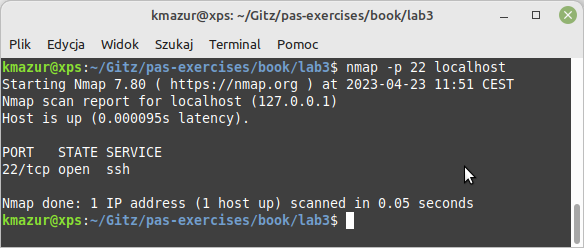
\includegraphics[scale=0.6]{./images/answers/ex3.1.png}
\end{figure}   
% #####################################################################################################

\item Możesz przetestować program używając swojego lokalnego adresu IPv6: \texttt{::1} lub \texttt{ip6-localhost} lub \\ \texttt{0000:0000:0000:0000:0000:0000:0000:0001}. 

\begin{figure}[h]
\caption{Wynik działania programu \texttt{nmap} dla lokalnej maszyny i portu \texttt{22}}
\centering
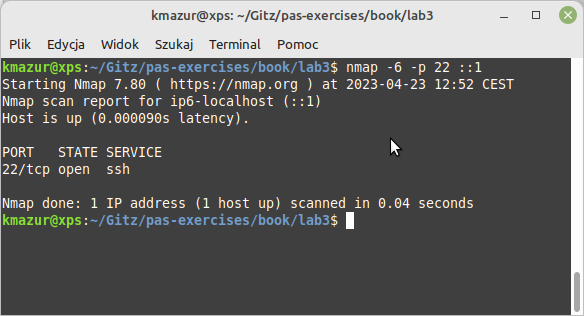
\includegraphics[scale=0.6]{./images/answers/ex3.2-nmap.png}
\end{figure}   
% #####################################################################################################

\newpage
\item Aby przetestować poprawność swojego rozwiązania, możesz przeskanować swój własny komputer, żeby sprawdzić, czy skanowanie da taki sam wynik, jak Twój program. Do tego celu możesz wykorzystać np. narzędzie \texttt{nmap}. Zainstaluj \texttt{nmap}: \texttt{sudo apt install nmap}, a następnie wydaj polecenie: \texttt{nmap -p1-65535 localhost} (lub \texttt{nmap -p1-65535 127.0.0.1}) aby sprawdzić, jakie porty są otwarte na Twoim komputerze. Porównaj wynik z działaniem Twojego programu dla tego samego portu.  

\begin{figure}[h]
\caption{Wynik działania programu \texttt{nmap} dla lokalnej maszyny i wszystkich jej portów}
\centering
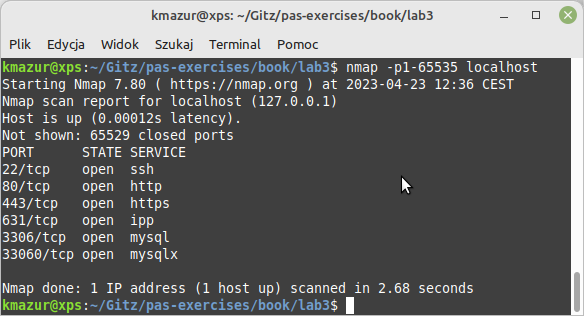
\includegraphics[scale=0.6]{./images/answers/ex3.3-nmap.png}
\end{figure}   
% #####################################################################################################

\item Aby przetestować poprawność swojego rozwiązania, możesz przeskanować swój własny komputer, żeby sprawdzić, czy skanowanie da taki sam wynik, jak Twój program. Do tego celu możesz wykorzystać np. narzędzie \texttt{nmap}. Zainstaluj \texttt{nmap}: \texttt{sudo apt install nmap}, a następnie wydaj polecenie: \texttt{nmap -6 -p1-65535 ip6-localhost} (lub \texttt{nmap -6 -p1-65535 ::1}) aby sprawdzić, jakie porty są otwarte na Twoim komputerze. Porównaj wynik z działaniem Twojego programu dla tego samego portu.  

\begin{figure}[h]
\caption{Wynik działania programu \texttt{nmap} dla lokalnej maszyny i wszystkich jej portów}
\centering
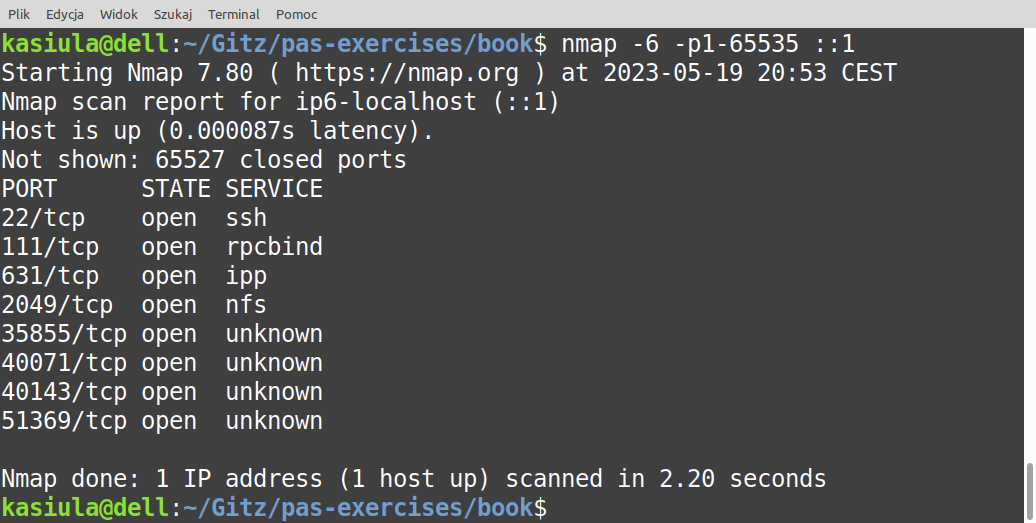
\includegraphics[scale=0.35]{./images/answers/ex3.4-nmap.png}
\end{figure}   
% #####################################################################################################

\item Aby przetestować poprawność swojego rozwiązania, możesz skorzystać z gotowego serwera, do którego może połączyć się Twój klient, aby pobrać aktualną datę i czas. Aby uruchomić serwer, zainstaluj \href{https://www.docker.com/}{Dockera}, a następnie w konsoli wydaj polecenia:

\begin{itemize}
\item Pobierz obraz serwera:\\ \texttt{docker pull mazurkatarzyna/pas-book-p1-ch3-ex5-server:latest}

\item Uruchom serwer za pomocą Dockera:\\ \texttt{docker run -dp 3005:3005 mazurkatarzyna/pas-book-p1-ch3-ex5-server}
\end{itemize}

\noindent Tak uruchomiony serwer działa na Twoim komputerze, jego adres IPv4 to \texttt{127.0.0.1} (\texttt{localhost}), numer portu to 3005.
% #####################################################################################################

\item Aby przetestować poprawność swojego rozwiązania, możesz skorzystać z gotowego serwera, do którego może połączyć się Twój klient, aby pobrać aktualną datę i czas. Aby uruchomić serwer, zainstaluj \href{https://www.docker.com/}{Dockera}, a następnie w konsoli wydaj polecenia:

\begin{itemize}
\item Pobierz obraz serwera:\\ \texttt{docker pull mazurkatarzyna/pas-book-p1-ch3-ex6-server:latest}

\item Uruchom serwer za pomocą Dockera:\\ \texttt{docker run -dp 3006:3006 mazurkatarzyna/pas-book-p1-ch3-ex6-server}
\end{itemize}

\noindent Tak uruchomiony serwer działa na Twoim komputerze, jego adres IPv6 to \texttt{::1} (\texttt{localhost}), numer portu to 3006.
% #####################################################################################################
\item Aby przetestować poprawność swojego rozwiązania, możesz skorzystać z gotowego serwera, do którego może połączyć się Twój klient, aby wysłać wiadomość. Aby uruchomić serwer, zainstaluj \href{https://www.docker.com/}{Dockera}, a następnie w konsoli wydaj polecenia:

\begin{itemize}
\item Pobierz obraz serwera:\\ \texttt{docker pull mazurkatarzyna/pas-book-p1-ch3-ex7-server:latest}

\item Uruchom serwer za pomocą Dockera:\\ \texttt{docker run -dp 3007:3007 mazurkatarzyna/pas-book-p1-ch3-ex7-server}
\end{itemize}

\noindent Tak uruchomiony serwer działa na Twoim komputerze, jego adres IPv4 to \texttt{127.0.0.1} (\texttt{localhost}), numer portu to 3007.
%#####################################################################################################

\item Aby przetestować poprawność swojego rozwiązania, możesz skorzystać z gotowego serwera, do którego może połączyć się Twój klient, aby wysłać wiadomość. Aby uruchomić serwer, zainstaluj \href{https://www.docker.com/}{Dockera}, a następnie w konsoli wydaj polecenia:

\begin{itemize}
\item Pobierz obraz serwera:\\ \texttt{docker pull mazurkatarzyna/pas-book-p1-ch3-ex8-server:latest}

\item Uruchom serwer za pomocą Dockera:\\ \texttt{docker run -dp 3008:3008 mazurkatarzyna/pas-book-p1-ch3-ex8-server}
\end{itemize}

\noindent Tak uruchomiony serwer działa na Twoim komputerze, jego adres IPv6 to \texttt{::1} (\texttt{localhost}), numer portu to 3008.
%#####################################################################################################
\item Aby przetestować poprawność swojego rozwiązania, możesz skorzystać z gotowego serwera, do którego może połączyć się Twój klient, aby wysłać wiadomość. Aby uruchomić serwer, zainstaluj \href{https://www.docker.com/}{Dockera}, a następnie w konsoli wydaj polecenia:

\begin{itemize}
\item Pobierz obraz serwera:\\ \texttt{docker pull mazurkatarzyna/pas-book-p1-ch3-ex9-server:latest}

\item Uruchom serwer za pomocą Dockera:\\ \texttt{docker run -dp 3009:3009 mazurkatarzyna/pas-book-p1-ch3-ex9-server}
\end{itemize}

\noindent Tak uruchomiony serwer działa na Twoim komputerze, jego adres IPv4 to \texttt{127.0.0.1} (\texttt{localhost}), numer portu to 3009.
%#####################################################################################################
\item Aby przetestować poprawność swojego rozwiązania, możesz skorzystać z gotowego serwera, do którego może połączyć się Twój klient, aby wysłać wiadomość. Aby uruchomić serwer, zainstaluj \href{https://www.docker.com/}{Dockera}, a następnie w konsoli wydaj polecenia:

\begin{itemize}
\item Pobierz obraz serwera:\\ \texttt{docker pull mazurkatarzyna/pas-book-p1-ch3-ex10-server:latest}

\item Uruchom serwer za pomocą Dockera:\\ \texttt{docker run -dp 3010:3010 mazurkatarzyna/pas-book-p1-ch3-ex10-server}
\end{itemize}

\noindent Tak uruchomiony serwer działa na Twoim komputerze, jego adres IPv6 to \texttt{::1} (\texttt{localhost}), numer portu to 3010.
%#####################################################################################################
 \item    Aby przetestować poprawność swojego rozwiązania, możesz przeskanować swój własny komputer, żeby sprawdzić, czy skanowanie da taki sam wynik, jak Twój program. Do tego celu możesz wykorzystać np. narzędzie \texttt{nmap} z parametrem \texttt{-{}-}\texttt{script=banner}. Zainstaluj \texttt{nmap}: \texttt{sudo apt install nmap}, a następnie wydaj polecenie: \texttt{nmap -p 22} \texttt{-{}-}\texttt{script=banner} \texttt{localhost} (lub \texttt{nmap -p 22} \texttt{-{}-}\texttt{script=banner} \texttt{127.0.0.1}) aby sprawdzić, czy port 22 jest otwarty na Twoim komputerze, i jaka usługa jest uruchomiona na tym porcie. Porównaj wynik z działaniem Twojego programu dla tego samego portu.  

\begin{figure}[h]
\caption{Wynik działania programu \texttt{nmap} dla lokalnej maszyny i portu \texttt{22}}
\centering
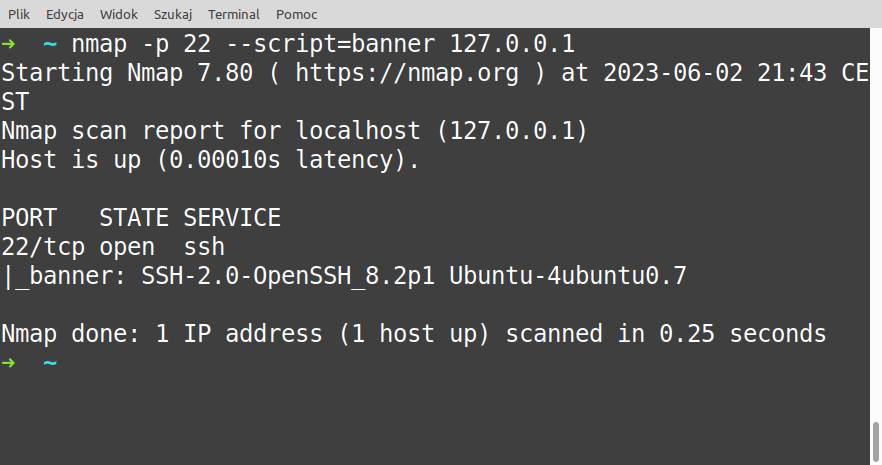
\includegraphics[scale=0.3]{./images/answers/ex3.11.png}
\end{figure}   
%#####################################################################################################
 \item    Aby przetestować poprawność swojego rozwiązania, możesz przeskanować swój własny komputer, żeby sprawdzić, czy skanowanie da taki sam wynik, jak Twój program. Do tego celu możesz wykorzystać np. narzędzie \texttt{nmap} z parametrem \texttt{-{}-}\texttt{script=banner}. Zainstaluj \texttt{nmap}: \texttt{sudo apt install nmap}, a następnie wydaj polecenie: \texttt{nmap -p 22 -6} \texttt{-{}-}\texttt{script=banner} \texttt{ip6-localhost} (lub \texttt{nmap -p 22 -6} \texttt{-{}-}\texttt{script=banner} \texttt{::1}) aby sprawdzić, czy port 22 jest otwarty na Twoim komputerze, i jaka usługa jest uruchomiona na tym porcie. Porównaj wynik z działaniem Twojego programu dla tego samego portu.  

\begin{figure}[h]
\caption{Wynik działania programu \texttt{nmap} dla lokalnej maszyny i portu \texttt{22}}
\centering
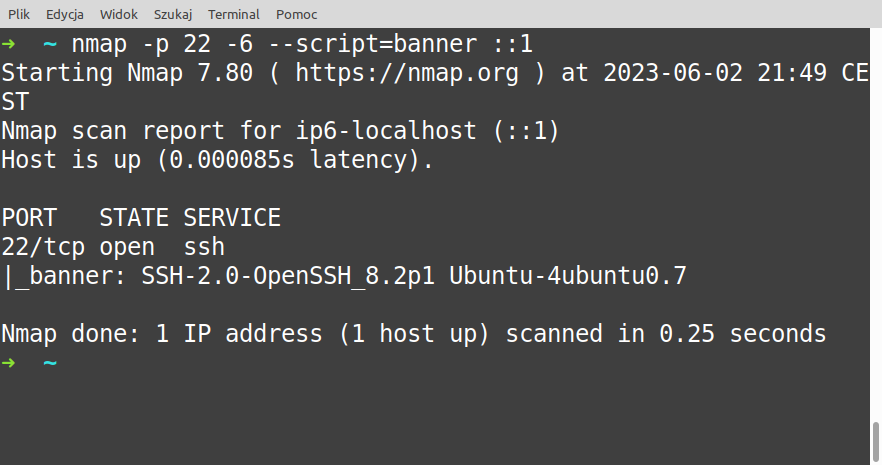
\includegraphics[scale=0.3]{./images/answers/ex3.12.png}
\end{figure}  
%#####################################################################################################
\item Aby przetestować poprawność swojego rozwiązania, możesz skorzystać z gotowego serwera, do którego może połączyć się Twój klient, aby wysłać wiadomość. Aby uruchomić serwer, zainstaluj \href{https://www.docker.com/}{Dockera}, a następnie w konsoli wydaj polecenia:

\begin{itemize}
\item Pobierz obraz serwera:\\ \texttt{docker pull mazurkatarzyna/pas-book-p1-ch3-ex13-server:latest}

\item Uruchom serwer za pomocą Dockera:\\ \texttt{docker run -dp 3013:3013 mazurkatarzyna/pas-book-p1-ch3-ex13-server}
\end{itemize}

\noindent Tak uruchomiony serwer działa na Twoim komputerze, jego adres IPv4 to \texttt{127.0.0.1} (\texttt{localhost}), numer portu to 3013.

\end{enumerate}
%#####################################################################################################
\newpage
\subsection*{Protokoły pocztowe - protokół SMTP}
\begin{enumerate}[label=\textbf{6.\arabic*}]\setlength{\itemsep}{1em}
\item \label{answ61} Do wykonania zadania możesz użyć:
\begin{itemize}
	\item Klienta \texttt{telnet}, jeśli serwer nie wymaga szyfrowania, polecenie do nawiązania połączenia z serwerem: \texttt{telnet server\_ip port}
	\item Klienta \texttt{OpenSSL}, o nazwie \texttt{s\_client} jeśli serwer wymaga szyfrowania, polecenie do nawiązania połączenia z serwerem: \texttt{openssl s\_client -crlf -connect server\_ip:port}
\end{itemize}
\noindent Jako serwera SMTP możesz użyć:
\begin{itemize}
 \item \texttt{iRedMail}, który dostępny jest jako \href{https://hub.docker.com/r/iredmail/mariadb}{kontener Dockerowy}, 
 \item Serwera pocztowego udostępnianego np. przez \texttt{interia.pl}, gdzie \texttt{poczta.interia.pl} jest adresem serwera SMTP, \texttt{465} jest numerem portu, na którym działa serwer. Potrzebujesz również konta na serwerze.
 \end{itemize}
 \noindent Poniżej przykład połączenia z serwerem \texttt{poczta.interia.pl}:
 \begin{figure}[h]
\centering
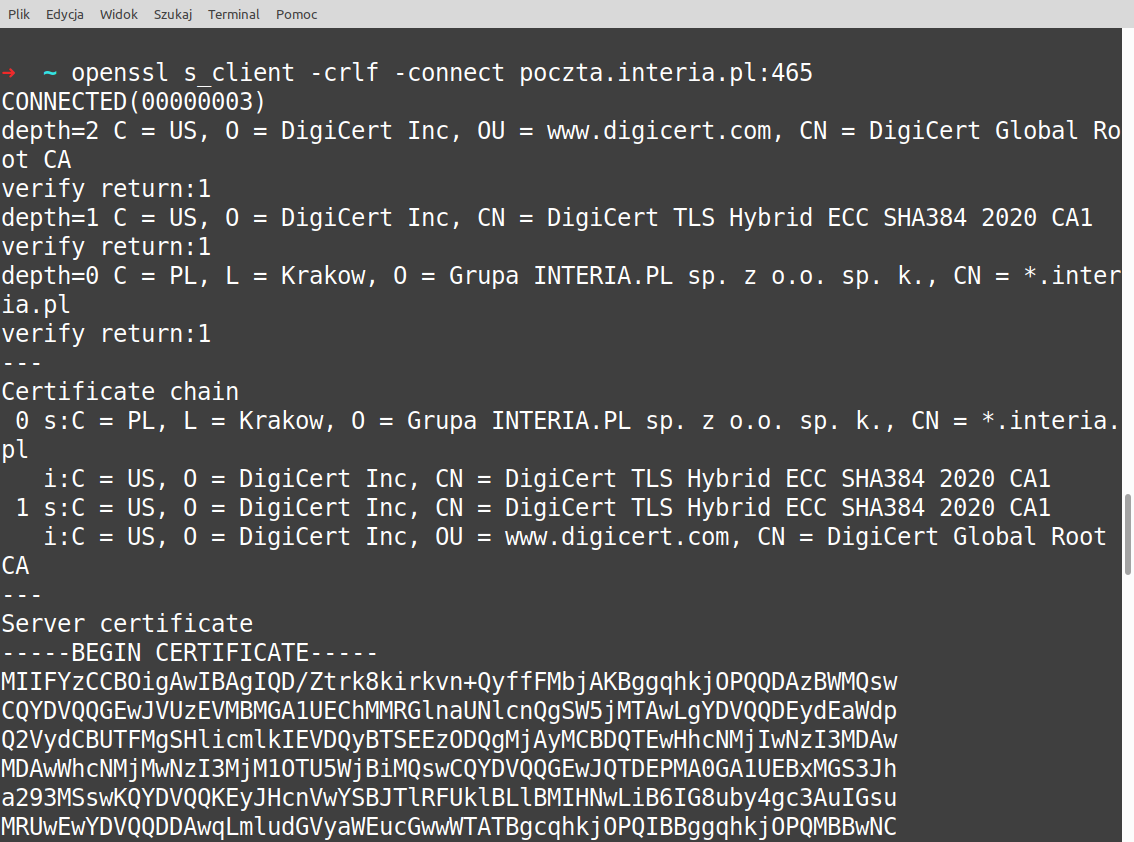
\includegraphics[scale=0.25]{./images/answers/smtp1.png}
\end{figure}  
 \begin{figure}[h]
\centering
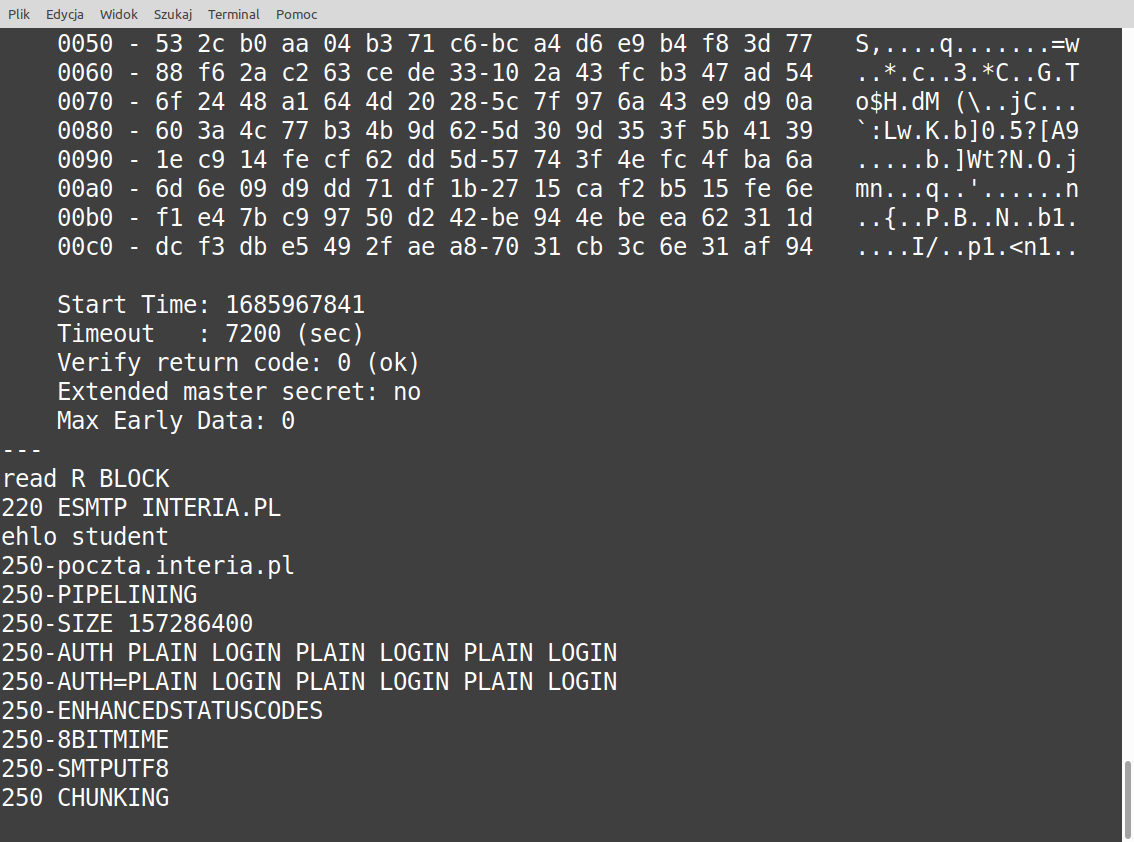
\includegraphics[scale=0.25]{./images/answers/smtp2.png}
\end{figure} 

\newpage 
\noindent Na niebiesko zaznaczono polecenia / komendy, których musisz użyć. Kolorem czarnym oznaczono odpowiedzi serwera:\\ \mbox{}
\scriptsize
\begin{alltt}
\textcolor{blue}{openssl s_client -crlf -connect poczta.interia.pl:465}
CONNECTED(00000003)
depth=2 C = US, O = DigiCert Inc, OU = www.digicert.com, CN = DigiCert Global Root CA
verify return:1
depth=1 C = US, O = DigiCert Inc, CN = DigiCert TLS Hybrid ECC SHA384 2020 CA1
verify return:1
depth=0 C = PL, L = Krakow, O = Grupa INTERIA.PL sp. z o.o. sp. k., CN = *.interia.pl
verify return:1
---
Certificate chain
 0 s:C = PL, L = Krakow, O = Grupa INTERIA.PL sp. z o.o. sp. k., CN = *.interia.pl
   i:C = US, O = DigiCert Inc, CN = DigiCert TLS Hybrid ECC SHA384 2020 CA1
 1 s:C = US, O = DigiCert Inc, CN = DigiCert TLS Hybrid ECC SHA384 2020 CA1
   i:C = US, O = DigiCert Inc, OU = www.digicert.com, CN = DigiCert Global Root CA
---
Server certificate
-----BEGIN CERTIFICATE-----
MIIFYzCCBOigAwIBAgIQD/Ztrk8kirkvn+QyffFMbjAKBggqhkjOPQQDAzBWMQsw
CQYDVQQGEwJVUzEVMBMGA1UEChMMRGlnaUNlcnQgSW5jMTAwLgYDVQQDEydEaWdp
Q2VydCBUTFMgSHlicmlkIEVDQyBTSEEzODQgMjAyMCBDQTEwHhcNMjIwNzI3MDAw
MDAwWhcNMjMwNzI3MjM1OTU5WjBiMQswCQYDVQQGEwJQTDEPMA0GA1UEBxMGS3Jh
a293MSswKQYDVQQKEyJHcnVwYSBJTlRFUklBLlBMIHNwLiB6IG8uby4gc3AuIGsu
MRUwEwYDVQQDDAwqLmludGVyaWEucGwwWTATBgcqhkjOPQIBBggqhkjOPQMBBwNC
AATj14S/K9d1aInT0/N6wXhyj7/0YxfJlR7jOxE8C5JiUZpaip8/DDL7syoNB3xS
LtJIpG1Ygqy9kRHr8wfIVOCzo4IDijCCA4YwHwYDVR0jBBgwFoAUCrwIKReMpTlt
eg7OM8cus+37w3owHQYDVR0OBBYEFEzd3VGbvBiH2K8Z1aE6Py9C0HHNMCMGA1Ud
EQQcMBqCDCouaW50ZXJpYS5wbIIKaW50ZXJpYS5wbDAOBgNVHQ8BAf8EBAMCB4Aw
HQYDVR0lBBYwFAYIKwYBBQUHAwEGCCsGAQUFBwMCMIGbBgNVHR8EgZMwgZAwRqBE
oEKGQGh0dHA6Ly9jcmwzLmRpZ2ljZXJ0LmNvbS9EaWdpQ2VydFRMU0h5YnJpZEVD
Q1NIQTM4NDIwMjBDQTEtMS5jcmwwRqBEoEKGQGh0dHA6Ly9jcmw0LmRpZ2ljZXJ0
LmNvbS9EaWdpQ2VydFRMU0h5YnJpZEVDQ1NIQTM4NDIwMjBDQTEtMS5jcmwwPgYD
VR0gBDcwNTAzBgZngQwBAgIwKTAnBggrBgEFBQcCARYbaHR0cDovL3d3dy5kaWdp
Y2VydC5jb20vQ1BTMIGFBggrBgEFBQcBAQR5MHcwJAYIKwYBBQUHMAGGGGh0dHA6
Ly9vY3NwLmRpZ2ljZXJ0LmNvbTBPBggrBgEFBQcwAoZDaHR0cDovL2NhY2VydHMu
ZGlnaWNlcnQuY29tL0RpZ2lDZXJ0VExTSHlicmlkRUNDU0hBMzg0MjAyMENBMS0x
LmNydDAJBgNVHRMEAjAAMIIBfQYKKwYBBAHWeQIEAgSCAW0EggFpAWcAdQCt9776
fP8QyIudPZwePhhqtGcpXc+xDCTKhYY069yCigAAAYJBhgsMAAAEAwBGMEQCIELl
g7IxBfCpgigx/rDU7kUvWaYWvMxf0tRkTL2UHbSVAiBIGwYMqfuFuoThbrny0stk
O4hwJoak4J69MvZ+HasnAQB2ADXPGRu/sWxXvw+tTG1Cy7u2JyAmUeo/4SrvqAPD
O9ZMAAABgkGGCtYAAAQDAEcwRQIhAPFjNAwBAB5v0G0Qw0uaDWMF7n3n/7s2t7gZ
Nlhy6Z8sAiBcLcCvAP/llzyfk/5olh01c85cWB6+HD3if6BUoUNMlgB2ALNzdwfh
hFD4Y4bWBancEQlKeS2xZwwLh9zwAw55NqWaAAABgkGGCwEAAAQDAEcwRQIgSsPk
X+yBkecqv0CuIXmWg9V2e/s4LYyYvsuIJU7ksxgCIQDkrabch4m6Sg9U6AaqeW8M
vPtFrIjAzwSymXt2lNyKTDAKBggqhkjOPQQDAwNpADBmAjEAv+cUUU3e9sdRaOFs
ntdpEVKb4S71HWCsVRZcS2MGIMOZRJ5LVEhhXHKl+EIaJ257AjEA8rSvrwL4MIRz
fCA70evopfs2fJcQVU4TLEbSFBwkAdh0LlHAnXH+NELH1ttjQtfh
-----END CERTIFICATE-----
subject=C = PL, L = Krakow, O = Grupa INTERIA.PL sp. z o.o. sp. k., CN = *.interia.pl

issuer=C = US, O = DigiCert Inc, CN = DigiCert TLS Hybrid ECC SHA384 2020 CA1

---
No client certificate CA names sent
Peer signing digest: SHA256
Peer signature type: ECDSA
Server Temp Key: X25519, 253 bits
---
SSL handshake has read 2811 bytes and written 389 bytes
Verification: OK
---
New, TLSv1.3, Cipher is TLS_AES_256_GCM_SHA384
Server public key is 256 bit
Secure Renegotiation IS NOT supported
Compression: NONE
Expansion: NONE
No ALPN negotiated
Early data was not sent
Verify return code: 0 (ok)
---
---
Post-Handshake New Session Ticket arrived:
SSL-Session:
    Protocol  : TLSv1.3
    Cipher    : TLS_AES_256_GCM_SHA384
    Session-ID: FA72D8E642670674F87A2BF7DE7D8716408D48DB0AF3F21F374FC989B6944C41
    Session-ID-ctx: 
    Resumption PSK: 
    328002BF74A3AC45B3D49DB69A6CEEBB80D17CFE1DE2BD71184A508001BABB1DC480C737B60DA4B6C43C40C1068039A2
    PSK identity: None
    PSK identity hint: None
    SRP username: None
    TLS session ticket lifetime hint: 7200 (seconds)
    TLS session ticket:
    0000 - d6 18 a0 85 49 b4 4b 4d-46 6d 71 b6 5f 38 ce 17   ....I.KMFmq._8..
    0010 - be e4 36 99 4d 17 4c ce-8b 13 6f 61 0b 3d e6 17   ..6.M.L...oa.=..
    0020 - 51 53 d6 d3 bf fc da 87-0f 38 eb 9c f0 fd 0e 5d   QS.......8.....]
    0030 - c0 9d 2f 95 e4 b3 78 24-98 b8 cd b4 83 50 08 43   ../...x\$.....P.C
    0040 - 1b e8 2b eb cd ee 3d 20-ef d6 4e 89 9d a6 21 92   ..+...= ..N...!.
    0050 - a7 0e 9b 04 e1 1e 9f 36-3f 6d 7b a5 a9 37 7d af   .......6?m\{..7\}.
    0060 - b4 3a 52 dc 68 7a 35 3b-89 74 89 ea ae 34 ba 46   .:R.hz5;.t...4.F
    0070 - fb e6 c6 da c3 f9 c1 89-f4 1e 89 28 50 32 12 74   ...........(P2.t
    0080 - 07 55 d0 7d 70 2f 1d e0-02 ca 6a e7 41 25 8f 53   .U.\}p/....j.A\%.S
    0090 - 5e 67 1d 25 f5 9f ab f9-e5 ce 0d 4d 05 78 46 4f   ^g.\%.......M.xFO
    00a0 - 11 d4 bb 3b 84 d2 26 71-28 3d 0b 13 a9 aa 85 95   ...;..&q(=......
    00b0 - 8d 77 c9 d0 be e5 d3 38-51 b1 1b f2 8b 9f 7e 8c   .w.....8Q.....~.
    00c0 - bb e9 5a f4 f9 71 40 3d-a1 1c 5b fe 35 c3 74 bf   ..Z..q@=..[.5.t.

    Start Time: 1685969504
    Timeout   : 7200 (sec)
    Verify return code: 0 (ok)
    Extended master secret: no
    Max Early Data: 0
---
read R BLOCK
220 ESMTP INTERIA.PL
\textcolor{blue}{ehlo student}
250-poczta.interia.pl
250-PIPELINING
250-SIZE 157286400
250-AUTH PLAIN LOGIN PLAIN LOGIN PLAIN LOGIN
250-AUTH=PLAIN LOGIN PLAIN LOGIN PLAIN LOGIN
250-ENHANCEDSTATUSCODES
250-8BITMIME
250-SMTPUTF8
250 CHUNKING
\textcolor{blue}{auth login}
334 VXNlcm5hbWU6
\textcolor{blue}{a29jaGFtLnVtY3NAaW50ZXJpYS5wbA==}
334 UGFzc3dvcmQ6
\textcolor{blue}{a29jaGFtLnVtY3MyMDIz}
235 2.7.0 Authentication successful
\textcolor{blue}{mail from: <kocham.umcs@interia.pl>}
250 2.1.0 Ok
\textcolor{blue}{rcpt to: <pas.umcs@poczta.fm>}
250 2.1.5 Ok
\textcolor{blue}{data}
354 End data with <CR><LF>.<CR><LF>
\textcolor{blue}{to: <pas.umcs@poczta.fm>}
\textcolor{blue}{from: <kocham.umcs@interia.pl>}    
\textcolor{blue}{subject: test email}

\textcolor{blue}{Hello!}

\textcolor{blue}{.}
250 OK. ID: 1054c830c3886b54
\textcolor{blue}{quit}
221 2.0.0 Bye
closed
\end{alltt}

\normalsize
\item Możesz skorzystać z jednego z serwerów SMTP zaproponowanego w rozwiązaniu do zadania \ref{answ61}. Jaka komenda protokołu SMTP pozwala na określenie odbiorcy wiadomości? 

\item Możesz skorzystać z jednego z serwerów SMTP zaproponowanego w rozwiązaniu do zadania \ref{answ61}. Jaka komenda protokołu SMTP pozwala na określenie nadawcy wiadomości? 

\item Możesz skorzystać z jednego z serwerów SMTP zaproponowanego w rozwiązaniu do zadania \ref{answ61}. Pamiętaj, że każda nowa linia ma znaczenie. Jeśli nie zachowasz odpowiedniej składni, serwer może ''nie zrozumieć'' wiadomości. Poniżej przykładowe rozwiązanie.  

\scriptsize
\begin{alltt}
\textcolor{blue}{openssl s_client -crlf -connect poczta.interia.pl:465}
CONNECTED(00000003)
depth=2 C = US, O = DigiCert Inc, OU = www.digicert.com, CN = DigiCert Global Root CA
verify return:1
depth=1 C = US, O = DigiCert Inc, CN = DigiCert TLS Hybrid ECC SHA384 2020 CA1
verify return:1
depth=0 C = PL, L = Krakow, O = Grupa INTERIA.PL sp. z o.o. sp. k., CN = *.interia.pl
verify return:1
---
Certificate chain
 0 s:C = PL, L = Krakow, O = Grupa INTERIA.PL sp. z o.o. sp. k., CN = *.interia.pl
   i:C = US, O = DigiCert Inc, CN = DigiCert TLS Hybrid ECC SHA384 2020 CA1
 1 s:C = US, O = DigiCert Inc, CN = DigiCert TLS Hybrid ECC SHA384 2020 CA1
   i:C = US, O = DigiCert Inc, OU = www.digicert.com, CN = DigiCert Global Root CA
---
Server certificate
-----BEGIN CERTIFICATE-----
MIIFYzCCBOigAwIBAgIQD/Ztrk8kirkvn+QyffFMbjAKBggqhkjOPQQDAzBWMQsw
CQYDVQQGEwJVUzEVMBMGA1UEChMMRGlnaUNlcnQgSW5jMTAwLgYDVQQDEydEaWdp
Q2VydCBUTFMgSHlicmlkIEVDQyBTSEEzODQgMjAyMCBDQTEwHhcNMjIwNzI3MDAw
MDAwWhcNMjMwNzI3MjM1OTU5WjBiMQswCQYDVQQGEwJQTDEPMA0GA1UEBxMGS3Jh
a293MSswKQYDVQQKEyJHcnVwYSBJTlRFUklBLlBMIHNwLiB6IG8uby4gc3AuIGsu
MRUwEwYDVQQDDAwqLmludGVyaWEucGwwWTATBgcqhkjOPQIBBggqhkjOPQMBBwNC
AATj14S/K9d1aInT0/N6wXhyj7/0YxfJlR7jOxE8C5JiUZpaip8/DDL7syoNB3xS
LtJIpG1Ygqy9kRHr8wfIVOCzo4IDijCCA4YwHwYDVR0jBBgwFoAUCrwIKReMpTlt
eg7OM8cus+37w3owHQYDVR0OBBYEFEzd3VGbvBiH2K8Z1aE6Py9C0HHNMCMGA1Ud
EQQcMBqCDCouaW50ZXJpYS5wbIIKaW50ZXJpYS5wbDAOBgNVHQ8BAf8EBAMCB4Aw
HQYDVR0lBBYwFAYIKwYBBQUHAwEGCCsGAQUFBwMCMIGbBgNVHR8EgZMwgZAwRqBE
oEKGQGh0dHA6Ly9jcmwzLmRpZ2ljZXJ0LmNvbS9EaWdpQ2VydFRMU0h5YnJpZEVD
Q1NIQTM4NDIwMjBDQTEtMS5jcmwwRqBEoEKGQGh0dHA6Ly9jcmw0LmRpZ2ljZXJ0
LmNvbS9EaWdpQ2VydFRMU0h5YnJpZEVDQ1NIQTM4NDIwMjBDQTEtMS5jcmwwPgYD
VR0gBDcwNTAzBgZngQwBAgIwKTAnBggrBgEFBQcCARYbaHR0cDovL3d3dy5kaWdp
Y2VydC5jb20vQ1BTMIGFBggrBgEFBQcBAQR5MHcwJAYIKwYBBQUHMAGGGGh0dHA6
Ly9vY3NwLmRpZ2ljZXJ0LmNvbTBPBggrBgEFBQcwAoZDaHR0cDovL2NhY2VydHMu
ZGlnaWNlcnQuY29tL0RpZ2lDZXJ0VExTSHlicmlkRUNDU0hBMzg0MjAyMENBMS0x
LmNydDAJBgNVHRMEAjAAMIIBfQYKKwYBBAHWeQIEAgSCAW0EggFpAWcAdQCt9776
fP8QyIudPZwePhhqtGcpXc+xDCTKhYY069yCigAAAYJBhgsMAAAEAwBGMEQCIELl
g7IxBfCpgigx/rDU7kUvWaYWvMxf0tRkTL2UHbSVAiBIGwYMqfuFuoThbrny0stk
O4hwJoak4J69MvZ+HasnAQB2ADXPGRu/sWxXvw+tTG1Cy7u2JyAmUeo/4SrvqAPD
O9ZMAAABgkGGCtYAAAQDAEcwRQIhAPFjNAwBAB5v0G0Qw0uaDWMF7n3n/7s2t7gZ
Nlhy6Z8sAiBcLcCvAP/llzyfk/5olh01c85cWB6+HD3if6BUoUNMlgB2ALNzdwfh
hFD4Y4bWBancEQlKeS2xZwwLh9zwAw55NqWaAAABgkGGCwEAAAQDAEcwRQIgSsPk
X+yBkecqv0CuIXmWg9V2e/s4LYyYvsuIJU7ksxgCIQDkrabch4m6Sg9U6AaqeW8M
vPtFrIjAzwSymXt2lNyKTDAKBggqhkjOPQQDAwNpADBmAjEAv+cUUU3e9sdRaOFs
ntdpEVKb4S71HWCsVRZcS2MGIMOZRJ5LVEhhXHKl+EIaJ257AjEA8rSvrwL4MIRz
fCA70evopfs2fJcQVU4TLEbSFBwkAdh0LlHAnXH+NELH1ttjQtfh
-----END CERTIFICATE-----
subject=C = PL, L = Krakow, O = Grupa INTERIA.PL sp. z o.o. sp. k., CN = *.interia.pl

issuer=C = US, O = DigiCert Inc, CN = DigiCert TLS Hybrid ECC SHA384 2020 CA1

---
No client certificate CA names sent
Peer signing digest: SHA256
Peer signature type: ECDSA
Server Temp Key: X25519, 253 bits
---
SSL handshake has read 2810 bytes and written 389 bytes
Verification: OK
---
New, TLSv1.3, Cipher is TLS_AES_256_GCM_SHA384
Server public key is 256 bit
Secure Renegotiation IS NOT supported
Compression: NONE
Expansion: NONE
No ALPN negotiated
Early data was not sent
Verify return code: 0 (ok)
---
---
Post-Handshake New Session Ticket arrived:
SSL-Session:
    Protocol  : TLSv1.3
    Cipher    : TLS_AES_256_GCM_SHA384
    Session-ID: F75D463B69633B1F1958D6CE033697EAC3AC78E1ABAA461599D03B4822ACCEE6
    Session-ID-ctx: 
    Resumption PSK: 74B14972C5CC86292F1A2869821072E8A55177841455905EE18CA32CC871922F62A95CCA9B68450180CCD5D937D57981
    PSK identity: None
    PSK identity hint: None
    SRP username: None
    TLS session ticket lifetime hint: 7200 (seconds)
    TLS session ticket:
    0000 - a9 09 45 e3 8a 1e 19 3c-8a f7 6c ae 0e 95 f1 62   ..E....<..l....b
    0010 - ac 28 8e 1c aa 29 02 42-86 75 c5 88 5e 2f f3 c6   .(...).B.u..^/..
    0020 - 44 87 f9 04 91 ce 7e 6c-1d 0f 18 9a be 7d 11 56   D.....~l.....\}.V
    0030 - 73 71 be 37 61 bd 3e 8c-64 d2 7f d4 3c 7b 90 ab   sq.7a.>.d...<\{..
    0040 - fd 63 f7 c6 dd d5 3b a6-d6 cf 08 35 d8 42 88 a8   .c....;....5.B..
    0050 - be 40 5b fa a9 a3 40 57-85 3d 5e 6c b6 d7 97 36   .@[...@W.=^l...6
    0060 - 4c 17 41 f1 d1 da e8 79-49 81 36 bc 95 5e 09 c4   L.A....yI.6..^..
    0070 - 88 78 16 99 b0 28 e5 12-30 aa 5f f9 35 ac 2a c8   .x...(..0._.5.*.
    0080 - 79 68 51 93 0d 5d 5c 50-1a 5a ed 84 7f ee c1 7a   yhQ..]\P.Z.....z
    0090 - 10 d9 50 81 4c 9c 7d 75-9b f5 33 d7 09 85 43 1c   ..P.L.\}u..3...C.
    00a0 - e0 54 ca e0 f9 bc 39 a3-55 c1 82 e2 82 96 a8 ef   .T....9.U.......
    00b0 - a3 99 6e 61 e7 a5 e0 7f-c8 e9 77 16 14 ad 08 81   ..na......w.....
    00c0 - dd 93 df 4f db 13 d5 d0-5d 74 7b 71 aa 12 26 a2   ...O....]t\{q..&.

    Start Time: 1685976897
    Timeout   : 7200 (sec)
    Verify return code: 0 (ok)
    Extended master secret: no
    Max Early Data: 0
---
read R BLOCK
220 ESMTP INTERIA.PL
\textcolor{blue}{ehlo student}
250-poczta.interia.pl
250-PIPELINING
250-SIZE 157286400
250-AUTH PLAIN LOGIN PLAIN LOGIN PLAIN LOGIN
250-AUTH=PLAIN LOGIN PLAIN LOGIN PLAIN LOGIN
250-ENHANCEDSTATUSCODES
250-8BITMIME
250-SMTPUTF8
250 CHUNKING
\textcolor{blue}{auth login}
334 VXNlcm5hbWU6
\textcolor{blue}{a29jaGFtLnVtY3NAaW50ZXJpYS5wbA==}
334 UGFzc3dvcmQ6
\textcolor{blue}{a29jaGFtLnVtY3MyMDIz}
235 2.7.0 Authentication successful
\textcolor{blue}{mail from: <kocham.umcs@interia.pl>}
250 2.1.0 Ok
\textcolor{blue}{rcpt to: <pas.umcs@poczta.fm>}
250 2.1.5 Ok
\textcolor{blue}{data}
354 End data with <CR><LF>.<CR><LF>
\textcolor{blue}{to: <pas.umcs@poczta.fm>}
\textcolor{blue}{from: <kocham.umcs@interia.pl>}
\textcolor{blue}{subject: test email}
\textcolor{blue}{MIME-Version: 1.0}
\textcolor{blue}{Content-Type: multipart/mixed; boundary=sep}

\textcolor{blue}{--sep}

\textcolor{blue}{To}
\textcolor{blue}{jest}
\textcolor{blue}{Tresc wiadomosci}
\textcolor{blue}{--sep}
\textcolor{blue}{Content-Type: text/x-log; name=text.log}
\textcolor{blue}{Content-Disposition: attachment; filename=text.log}
\textcolor{blue}{Content-Transfer-Encoding: base64}
\textcolor{blue}{SGVsbG8K}
\textcolor{blue}{--sep--}
\textcolor{blue}{.}
250 OK. ID: bb63e06c9c318562
\textcolor{blue}{quit}
221 2.0.0 Bye
closed
\end{alltt}
\normalsize

\noindent Po sprawdzeniu swojej skrzynki pocztowej, powinieneś zobaczyć wysłaną wiadomość wraz z załącznikiem: \\

 \begin{figure}[h]
\centering
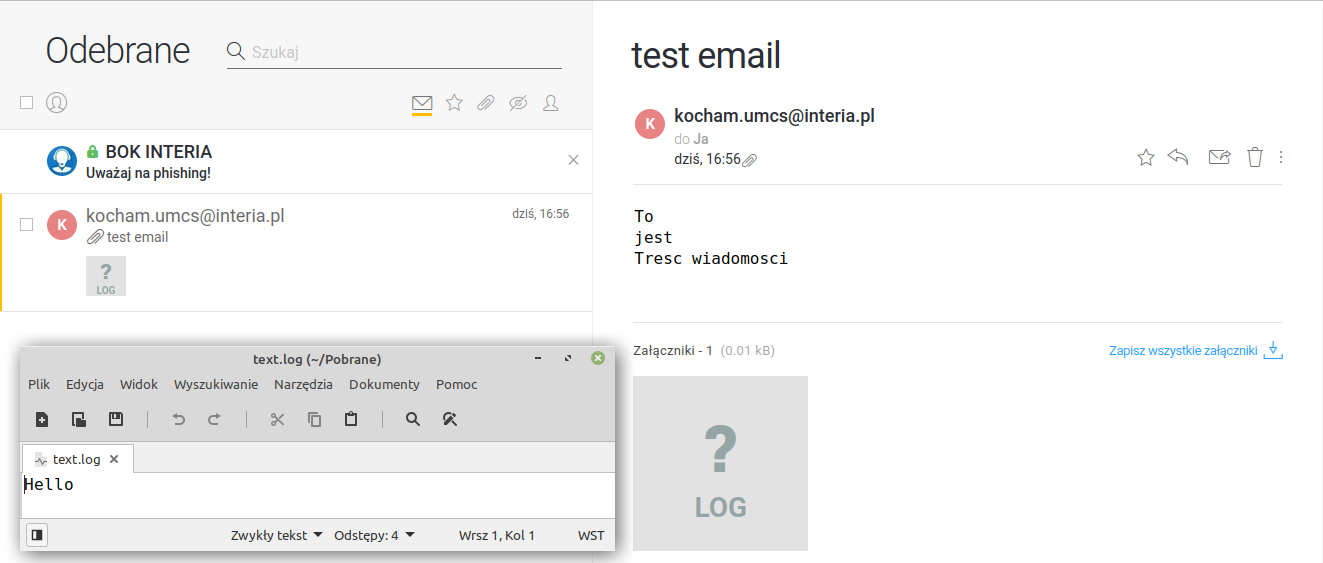
\includegraphics[scale=0.35]{./images/answers/email1.png}
\end{figure} 

\item Możesz skorzystać z jednego z serwerów SMTP zaproponowanego w rozwiązaniu do zadania \ref{answ61}. Pamiętaj, że każda nowa linia ma znaczenie. Jeśli nie zachowasz odpowiedniej składni, serwer może ''nie zrozumieć'' wiadomości. Poniżej przykładowe rozwiązanie.  

\scriptsize
\begin{verbatim}
telnet interia.pl 587
Trying 217.74.65.23...
Connected to interia.pl.
Escape character is '^]'.
220 ESMTP INTERIA.PL
HELO student
AUTH LOGIN
cGFzMjAxN0BpbnRlcmlhLnBs
UDRTSW5mMjAxNw==
MAIL FROM: <pas2017@interia.pl>
RCPT TO: <pas2017@interia.pl>
RCPT TO: <kasiula.mazur@gmail.com>
DATA

From: Nathaniel Borenstein <nsb@bellcore.com> 
To:  Ned Freed <ned@innosoft.com> 
Subject: Sample message 
MIME-Version: 1.0 
Content-Type: multipart/mixed; boundary=sep

--sep 

tresc wiadomosci
--sep
Content-Type: application/octet-stream; name=\"image.png\"
Content-Disposition: attachment; filename=\"image.png\"
Content-Transfer-Encoding: base64

/9j/4AAQSkZJRgABAQAAAQABAAD//gA7Q1JFQVRPUjogZ2QtanBlZyB2MS4wICh1
c2luZyBJSkcgSlBFRyB2NjIpLCBxdWFsaXR5ID0gODAK/9sAQwAGBAUGBQQGBgUG
BwcGCAoQCgoJCQoUDg8MEBcUGBgXFBYWGh0lHxobIxwWFiAsICMmJykqKRkfLTAt
KDAlKCko/9sAQwEHBwcKCAoTCgoTKBoWGigoKCgoKCgoKCgoKCgoKCgoKCgoKCgo
KCgoKCgoKCgoKCgoKCgoKCgoKCgoKCgoKCgo/8AAEQgGLgS9AwEiAAIRAQMRAf/E
...
--sep--
.
250 OK. ID: 1054c830c3886b54
QUIT
221 2.0.0 Bye
closed
\end{verbatim}
\normalsize

\newpage 
\item Możesz skorzystać z jednego z serwerów SMTP zaproponowanego w rozwiązaniu do zadania \ref{answ61}. Poniżej przykład nawiązania połączenia z serwerem (połączenie szyfrowane), i odebrania od serwera pierwszej wiadomości po połączeniu: \\  

\begin{figure}[h]
%\caption{Wynik działania programu \texttt{nmap} dla lokalnej maszyny i portu \texttt{22}}
\centering
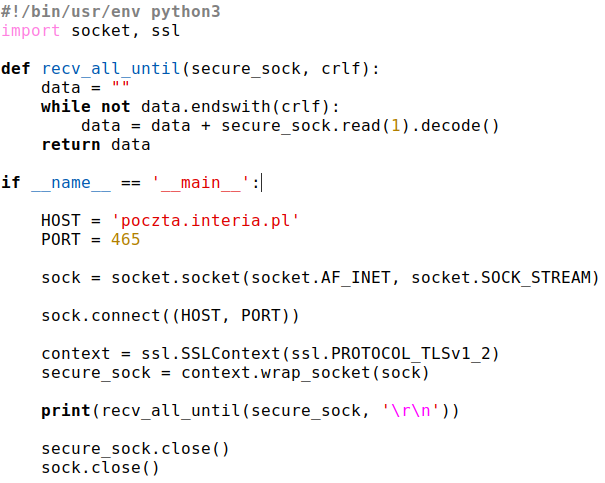
\includegraphics[scale=0.45]{./images/answers/smtp-py.png}
\end{figure}  

\item Możesz skorzystać z jednego z serwerów SMTP zaproponowanego w rozwiązaniu do zadania \ref{answ61}. 

\end{enumerate}

%#####################################################################################################
\newpage
\subsection*{Protokół HTTP}

\begin{enumerate}[label=\textbf{7.\arabic*}]\setlength{\itemsep}{1em}
\item Serwer możesz uruchomić za pomocą poniższych poleceń:

\begin{verbatim}
docker pull mazurkatarzyna/pas-book-p1-ch7-ex1:latest
docker run -dp 7001:80 mazurkatarzyna/pas-book-p1-ch7-ex1
\end{verbatim}

\noindent Działanie serwera możesz przetestować za pomocą przeglądarki. W swojej przeglądarce otwórz stronę: \url{http://127.0.0.1:7001/html} i podejrzyj, jak wygląda żądanie i odpowiedź HTTP.

% #################################################################################################################
\item Serwer możesz uruchomić za pomocą poniższych poleceń:

\begin{verbatim}
docker pull mazurkatarzyna/pas-book-p1-ch7-ex2:latest
docker run -dp 7002:80 mazurkatarzyna/pas-book-p1-ch7-ex2
\end{verbatim}

\noindent Działanie serwera możesz przetestować za pomocą przeglądarki. W swojej przeglądarce otwórz stronę: \url{http://127.0.0.1:7002/image/png} i podejrzyj, jak wygląda żądanie i odpowiedź HTTP.

% #################################################################################################################
\item Serwer możesz uruchomić za pomocą poniższych poleceń:

\begin{verbatim}
docker pull mazurkatarzyna/pas-book-p1-ch7-ex3:latest
docker run -dp 7003:80 mazurkatarzyna/pas-book-p1-ch7-ex3
\end{verbatim}

\noindent Działanie serwera możesz przetestować za pomocą przeglądarki. W swojej przeglądarce otwórz stronę: \url{http://127.0.0.1:7003/image.jpg} i podejrzyj, jak wygląda żądanie i odpowiedź HTTP.

% #################################################################################################################
\item Serwer możesz uruchomić za pomocą poniższych poleceń:

\begin{verbatim}
docker pull mazurkatarzyna/pas-book-p1-ch7-ex4:latest
docker run -dp 7004:80 mazurkatarzyna/pas-book-p1-ch7-ex4
\end{verbatim}

\noindent Działanie serwera możesz przetestować za pomocą przeglądarki. W swojej przeglądarce otwórz stronę: \url{http://127.0.0.1:7004/post} i podejrzyj, jak wygląda żądanie i odpowiedź HTTP.
% #################################################################################################################
\item Serwer możesz uruchomić za pomocą poniższych poleceń:

\begin{verbatim}
docker pull mazurkatarzyna/pas-book-p1-ch7-ex5:latest
docker run -dp 7005:80 mazurkatarzyna/pas-book-p1-ch7-ex5
\end{verbatim}

\noindent Działanie serwera możesz przetestować za pomocą przeglądarki. W swojej przeglądarce otwórz stronę: \url{http://127.0.0.1:7005}. Działający serwer powinien wyświetlać obrazek. W przypadku ataku DDoS, serwer będzie miał trudności w załadowaniu strony. Aby przetestować, czy Twój atak DDoS typu Slowloris jest skuteczny, możesz wykorzystać gotowe narzędzia, np. \url{https://github.com/gkbrk/slowloris} i zaatakować serwer.

% #################################################################################################################

\item 

\item \addtocounter{enumi}{3} Serwer możesz uruchomić za pomocą poniższych poleceń:

\begin{verbatim}
docker pull mazurkatarzyna/pas-book-p1-ch7-ex3:latest
docker run -dp 7003:80 mazurkatarzyna/pas-book-p1-ch7-ex3
\end{verbatim}

\noindent Działanie serwera możesz przetestować za pomocą przeglądarki. W swojej przeglądarce otwórz stronę: \url{http://127.0.0.1:7003/image.jpg} i podejrzyj, jak wygląda żądanie i odpowiedź HTTP.
% #################################################################################################################
\item Serwer możesz uruchomić za pomocą poniższych poleceń:

\begin{verbatim}
docker pull mazurkatarzyna/pas-book-p1-ch7-ex11:latest
docker run -dp 70011:7011 mazurkatarzyna/pas-book-p1-ch7-ex11
\end{verbatim}

\noindent Działanie serwera możesz przetestować za pomocą przeglądarki. W swojej przeglądarce otwórz stronę: \url{http://127.0.0.1:7011/?key=value} i podejrzyj, jak wygląda żądanie i odpowiedź HTTP.
% #################################################################################################################
\item Sprawdź manual narzędzia \texttt{cURL}: \texttt{man curl}.
% #################################################################################################################
\item Serwer możesz uruchomić za pomocą poniższych poleceń:

\begin{verbatim}
docker pull mazurkatarzyna/pas-book-p1-ch7-ex13:latest
docker run -dp 70013:7013 mazurkatarzyna/pas-book-p1-ch7-ex13
\end{verbatim}

\noindent Gdy serwer jest uruchomiony, spróbuj na początku wysłać do niego request za pomocą narzędzia \texttt{cURL}. 
% #################################################################################################################
\item Sprawdź manual narzędzia \texttt{cURL}: \texttt{man curl}.
% #################################################################################################################
\item Serwer możesz uruchomić za pomocą poniższych poleceń:

\begin{verbatim}
docker pull mazurkatarzyna/pas-book-p1-ch7-ex11:latest
docker run -dp 70011:7011 mazurkatarzyna/pas-book-p1-ch7-ex11
\end{verbatim}

\noindent Działanie serwera możesz przetestować za pomocą przeglądarki. W swojej przeglądarce otwórz stronę: \url{http://127.0.0.1:7011} i podejrzyj, jak wygląda żądanie i odpowiedź HTTP.
% #################################################################################################################
\item Sprawdź manual narzędzia \texttt{cURL}: \texttt{man curl}.
% #################################################################################################################
\item Serwer możesz uruchomić za pomocą poniższych poleceń:

\begin{verbatim}
docker pull mazurkatarzyna/pas-book-p1-ch7-ex11:latest
docker run -dp 70011:7011 mazurkatarzyna/pas-book-p1-ch7-ex11
\end{verbatim}

\noindent Działanie serwera możesz przetestować za pomocą przeglądarki. W swojej przeglądarce otwórz stronę: \url{http://127.0.0.1:7011} i podejrzyj, jak wygląda żądanie i odpowiedź HTTP. \\

 \noindent Przy rozwiązaniu zadania pomocna może być również wiedza o  \href{https://www.w3schools.com/tags/ref_urlencode.ASP}{kodowaniu URL}.  Przeglądarki internetowe żądają stron z serwerów sieciowych za pomocą adresu URL. Adres URL to adres strony internetowej, na przykład: \texttt{https://www.umcs.pl}. Kodowanie adresów URL (URL Encoding lub Percent Encoding) konwertuje znaki na format, który można przesyłać przez Internet. Adresy URL można przesyłać przez Internet tylko przy użyciu zestawu znaków ASCII. Ponieważ adresy URL często zawierają znaki spoza zestawu ASCII, adres URL musi zostać przekonwertowany na prawidłowy format ASCII. Kodowanie adresu URL zastępuje niebezpieczne znaki ASCII znakiem \texttt{\%}, po którym następują dwie cyfry szesnastkowe. Adresy URL nie mogą zawierać spacji. Kodowanie adresów URL zwykle zastępuje spację znakiem plus \texttt{+} lub \texttt{\%20}. Aby sprawdzić,  w jaki sposób w zapisie szesnastkowym można zakodować znak \texttt{\&}, możesz użyć narzędzia \texttt{ascii}. Wydaj polecenie \texttt{man ascii} aby sprawdzić manual narzędzia.
% #################################################################################################################
\item  Sprawdź manual narzędzia \texttt{cURL}: \texttt{man curl}. Pomocne będzie również użycie narzędzia \texttt{ascii}. Wydaj polecenie \texttt{man ascii} aby sprawdzić manual narzędzia.
% #################################################################################################################
\item Serwer możesz uruchomić za pomocą poniższych poleceń:

\begin{verbatim}
docker pull mazurkatarzyna/pas-book-p1-ch7-ex19:latest
docker run -dp 70019:7019 mazurkatarzyna/pas-book-p1-ch7-ex19
\end{verbatim}

\noindent Działanie serwera możesz przetestować za pomocą przeglądarki. W swojej przeglądarce otwórz stronę: \url{http://127.0.0.1:7019} i podejrzyj, jak wygląda żądanie i odpowiedź HTTP. Aby sprawdzić,  w jaki sposób w zapisie szesnastkowym można zakodować znak \texttt{?}, możesz użyć narzędzia \texttt{ascii}. Wydaj polecenie \texttt{man ascii} aby sprawdzić manual narzędzia.
% #################################################################################################################
\item Sprawdź manual narzędzia \texttt{cURL}: \texttt{man curl}. Pomocne będzie również użycie narzędzia \texttt{ascii}. Wydaj polecenie \texttt{man ascii} aby sprawdzić manual narzędzia.
% #################################################################################################################
\item Serwer możesz uruchomić za pomocą poniższych poleceń:

\begin{verbatim}
docker pull mazurkatarzyna/pas-book-p1-ch7-ex11:latest
docker run -dp 7011:7011 mazurkatarzyna/pas-book-p1-ch7-ex11
\end{verbatim}

\noindent Działanie serwera możesz przetestować za pomocą przeglądarki. W swojej przeglądarce otwórz stronę: \url{http://127.0.0.1:7011} i podejrzyj, jak wygląda żądanie i odpowiedź HTTP. Aby sprawdzić,  w jaki sposób w zapisie szesnastkowym można zakodować znak spacji, możesz użyć narzędzia \texttt{ascii}. Wydaj polecenie \texttt{man ascii} aby sprawdzić manual narzędzia.
% #################################################################################################################
\item Sprawdź manual narzędzia \texttt{cURL}: \texttt{man curl}. Pomocne będzie również użycie narzędzia \texttt{ascii}. Wydaj polecenie \texttt{man ascii} aby sprawdzić manual narzędzia.
% #################################################################################################################

\item Serwer możesz uruchomić za pomocą poniższych poleceń:

\begin{verbatim}
docker pull mazurkatarzyna/pas-book-p1-ch7-ex11:latest
docker run -dp 7011:7011 mazurkatarzyna/pas-book-p1-ch7-ex11
\end{verbatim}

\noindent Działanie serwera możesz przetestować za pomocą przeglądarki. W swojej przeglądarce otwórz stronę: \url{http://127.0.0.1:7011} i podejrzyj, jak wygląda żądanie i odpowiedź HTTP. Aby sprawdzić,  w jaki sposób w zapisie szesnastkowym można zakodować znak \texttt{\#}, możesz użyć narzędzia \texttt{ascii}. Wydaj polecenie \texttt{man ascii} aby sprawdzić manual narzędzia.
% #################################################################################################################
\item Sprawdź manual narzędzia \texttt{cURL}: \texttt{man curl}. Pomocne będzie również użycie narzędzia \texttt{ascii}. Wydaj polecenie \texttt{man ascii} aby sprawdzić manual narzędzia.
% #################################################################################################################
\item  Serwer możesz uruchomić za pomocą poniższych poleceń:

\begin{verbatim}
docker pull mazurkatarzyna/pas-book-p1-ch7-ex25:latest
docker run -dp 7025:7025 mazurkatarzyna/pas-book-p1-ch7-ex25
\end{verbatim}

\noindent Działanie serwera możesz przetestować za pomocą przeglądarki. W swojej przeglądarce otwórz stronę: \url{http://127.0.0.1:7025} i podejrzyj, jak wygląda żądanie i odpowiedź HTTP. Możesz użyć również narzędzia \texttt{ascii}. Wydaj polecenie \texttt{man ascii} aby sprawdzić manual narzędzia. \textit{Podpowiedź: Aby wysłać parametr jako tablicę, możesz użyć następującej składni:} \texttt{key[0]=value1\&key[1]=value2}.

% #################################################################################################################
\item Sprawdź manual narzędzia \texttt{cURL}: \texttt{man curl}. Aby wysłać parametr jako tablicę, możesz użyć następującej składni:  \texttt{key[0]=value1\&key[1]=value2}.
% #################################################################################################################
\item Sprawdź manual narzędzia \texttt{cURL}: \texttt{man curl}. Aby wysłać parametr jako tablicę, możesz użyć następującej składni:  \texttt{key[0]=value1\&key[1]=value2}. Aby sprawdzić,  w jaki sposób w zapisie szesnastkowym można zakodować znaki \texttt{[} oraz \texttt{]}, możesz użyć narzędzia \texttt{ascii}. Wydaj polecenie \texttt{man ascii} aby sprawdzić manual narzędzia.
% #################################################################################################################
 


\end{enumerate}

%\begin{enumerate}[label=\textbf{7.\arabic*}]\setlength{\itemsep}{1em}
%\end{enumerate}



\end{document}